\scanpage{8}
Supposons que $q\alpha-\alpha'\ne0$ alors
\[
\begin{aligned}
(1)\ \Longrightarrow\quad &p\mid\sum_{i=1}^{q-1}C_q^i\,a^i b'^{\,q-i-1}+b'^{\,q-1}\\
\Longrightarrow\quad &p\mid q\,a^{q-1}\qquad\text{car }p\mid b'\ \text{et pour }i\ne q-1\quad q-i-1\deleted{\ne0}>0
\end{aligned}
\]
or $p\mid b'$ et $b'\mid b^q$ donc $b'\mathrel{\underset{1}{\smile}}a$ donc $p\mathrel{\underset{1}{\smile}}a$

\deleted{donc si $\unsure{p\ne1|p\ne q}$}
\[
(1)\ \Longrightarrow\quad p\mid q\qquad\text{donc }\deleted{p=1\ \text{ou }}p=q\quad(\text{si }q\alpha-\alpha'\ne0)
\]
Donc si $p\ne q$ \quad $p$ premier \inserted{ou $p=1$} et $p\mid b'$ alors $\alpha'=q\alpha$
\begin{flushright}
\begin{tikzpicture}[baseline=(p.base)]
\node[inner sep=0pt] (p) at(0,0) {$\left(\begin{aligned}
&\text{\rlap{on l'impose sans risque}\phantom{\deleted{on l'impose sans risque}}}\\
&\quad\text{\rlap{si $p=1$}\phantom{\deleted{si $p=1$}}}
\end{aligned}\right)$};
\draw ([xshift=.05cm,yshift=-.03cm]p.south west) -- ([xshift=.08cm,yshift=.03cm]p.north);
\draw ([xshift=.22cm,yshift=-.04cm]p.south) -- ([xshift=-.04cm,yshift=.03cm]p.north east);
\end{tikzpicture}
\end{flushright}

Donc $\exists\,b_0\in\mathbb N^*$ et $\exists\,\gamma\in\mathbb N$ tel que $b'=q^\gamma b_0^q$ \margin{$q\nmid b_0$}

de plus $b_0\mid b$ et si $b=b_0 b''$ alors $b_0\mathrel{\underset{1}{\smile}}b''$ ?

De même $\exists\,a_0\in\mathbb N^*$ et $\exists\,\unsure{\zeta|\delta}\in\mathbb N$ tel que $a'=q^\zeta a_0^q$ avec $a_0\mid a$ et si $\overset{\unsure{\cdot|\prime}}{a}=a_0a''$ alors $a_0\mathrel{\underset{1}{\smile}}a''$ ?
% The small detached mark above a is positioned as seen; its role and hand remain open.

or $a\mathrel{\underset{1}{\smile}}b\Longrightarrow a_{\deleted{\unsure{0}}}'\mathrel{\underset{1}{\smile}}b'\Longrightarrow\zeta\times\gamma=0$ (et aussi $a_0\mathrel{\underset{1}{\smile}}b_0$)

Je suppose désormais que $\zeta=0$ donc $a'=a_0^q$

\figure{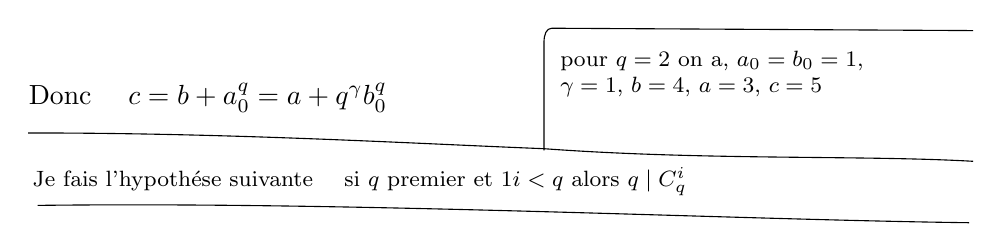
\begin{tikzpicture}[x=1cm,y=1cm]
\node[anchor=west,inner sep=0pt] at(0,.75) {Donc \quad $c=b+a_0^q=a+q^\gamma b_0^q$};
\node[anchor=west,inner sep=0pt,align=left,font=\footnotesize] at(6.75,1.05) {pour $q=2$ on a, $a_0=b_0=1$,\\$\gamma=1$, $b=4$, $a=3$, $c=5$};
\draw (12.0,1.60) -- (6.65,1.63) .. controls(6.58,1.63) and(6.55,1.55) .. (6.55,1.45) -- (6.55,.08);
\draw (0,.30) .. controls(2.6,.30) and(4.8,.17) .. (6.55,.10) .. controls(8.6,-.05) and(10.6,.02) .. (12.0,-.06);
\node[anchor=west,inner sep=0pt,font=\footnotesize] at(.05,-.32) {Je fais l'hypothése suivante \quad si $q$ premier et $1\leqslant i<q$ alors $q\mid C_q^i$};
\draw (.12,-.62) .. controls(4.2,-.57) and(8.9,-.80) .. (11.95,-.84);
\end{tikzpicture}}

alors Si $q\geqslant3$ et $q\alpha-\alpha'\geqslant2$ \deleted{alors} on a \inserted{$p=q,\ {\unsure{a|\alpha}}'=\gamma$}
\[
\begin{aligned}
(1)\ \Longrightarrow\quad &\deleted{\unsure{p^{2}|p}}q^2\mid q\,a^{q-1}\quad
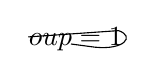
\begin{tikzpicture}[baseline=(d.base)]
\node[inner sep=0pt] (d) {\rlap{$\text{ou }p=1$}\phantom{$\deleted{\text{ou }p=1}$}};
\draw ([yshift=.03cm]d.west) -- ([yshift=.11cm,xshift=-.06cm]d.east)
 .. controls([xshift=.15cm,yshift=.04cm]d.east) and([xshift=.02cm,yshift=-.14cm]d.east)
 .. ([xshift=.24cm,yshift=-.10cm]d.center) -- ([xshift=-.06cm,yshift=-.06cm]d.center);
\end{tikzpicture}\\[.7ex]
\Longrightarrow\quad&q\mid a^{q-1}\quad
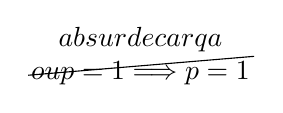
\begin{tikzpicture}[baseline=(d.base)]
\node[inner sep=0pt] (d) {\rlap{$\text{ou }p=1\Longrightarrow p=1$}\phantom{$\deleted{\text{ou }p=1\Longrightarrow p=1}$}};
\draw ([xshift=-.03cm,yshift=-.02cm]d.west) -- ([xshift=.05cm,yshift=.22cm]d.east);
\node[anchor=south,inner sep=0pt] at([yshift=.11cm]d.north) {$\inserted{\text{absurde car }q\nmid a}$};
\end{tikzpicture}
\end{aligned}
\]
Donc $\gamma=0$ ou $\gamma=
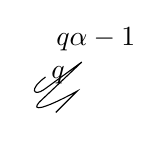
\begin{tikzpicture}[baseline=(q.base)]
\node[inner sep=0pt] (q) at(0,0) {\rlap{$q$}\phantom{$\deleted{q}$}};
\node[anchor=base west,inner sep=0pt] at(-.03,.38) {$q\alpha-1$};
\draw (-.16,-.02) .. controls(-.38,-.18) and(-.31,-.27) .. (-.18,-.18) -- (.30,.17)
 -- (-.24,-.34) .. controls(-.34,-.45) and(-.22,-.45) .. (.24,-.20) -- (-.03,-.47);
\end{tikzpicture}$ (sous réserve que l'hypothése est vraie)%
% The raised q alpha - 1 and the cancelled lower q are reproduced geometrically.
\margin{\begin{tikzpicture}[baseline=(n.base)]
\node[inner sep=0pt,text width=.85\marginparwidth] (n) {C'est peut-être interessant car ici $2$ est mis à part dans l'ensemble des nombres premiers};
\fill ([xshift=.07cm,yshift=-.47cm]n.south east) circle(.022cm);
\draw ([xshift=.15cm,yshift=-.47cm]n.south east) -- ([xshift=.31cm,yshift=-.47cm]n.south east)
 -- ([xshift=.35cm,yshift=-.16cm]n.north east)
 .. controls([xshift=.35cm,yshift=-.03cm]n.north east) and([xshift=.19cm,yshift=-.01cm]n.north east)
 .. ([xshift=.06cm,yshift=.01cm]n.north east);
\draw ([xshift=.19cm,yshift=.14cm]n.north east) .. controls([xshift=.00cm,yshift=.04cm]n.north east) and([xshift=-.01cm,yshift=-.06cm]n.north east) .. ([xshift=.15cm,yshift=-.10cm]n.north east);
\end{tikzpicture}}
% archive sheet number: 7
